\section{Results}
\label{sect:results}
\subsection{Experimental Design}
\label{subsect:experimental-design}

We conducted all experiments on a computer equipped with an Intel Core i5-7200U processor, 8 GB RAM, running Ubuntu 22.04 64-bit, and an NVIDIA GeForce GT 940MX GPU.

For image rendering, we utilized a classical volume ray-casting algorithm with Blinn-Phong illumination and trilinear interpolation. The ray step was adjusted according to voxel spacing. Our runtime analysis reflects the average of five trials.

The system was implemented in C++, using the Qt Framework and CUDA C/C++ for parallel processing. The implementation is available in online repositories.
%The system was implemented\footnotemark in C++, using the Qt Framework and CUDA C/C++ for parallel processing. The implementation is available in online repositories.
% \footnotetext{An implementation is available at \url{https://github.com/rafaelssantos/volumeexplorer}.}

Table~\ref{tab:datasets-descriptions} presents the datasets used in our experiments. These datasets are widely recognized within the volume visualization community and are publicly available through online repositories.

All volume data consisted solely of material density, represented as scalar intensity values. Since multidimensional data was not directly available, derived attribute extraction was performed to generate a multidimensional input. We considered 13 attributes, namely: intensity, gradient magnitude, Laplacian magnitude, and 10 statistical measures computed from a local histogram. The statistical measures include absolute deviation, contrast, energy, entropy, inertia, kurtosis, mean, skewness, standard deviation, and variance.


The selection of attributes for each dataset was conducted empirically. For each case, we evaluated which combination of derived attributes contributed most effectively to distinguishing relevant structures within the volume. This empirical approach allowed us to adapt the feature set to the specific characteristics of each dataset, ensuring a balance between discriminative power and computational efficiency.


\begin{table}[htb!]
    \centering
    \caption{Volume datasets.}
    \begin{tabular}{@{}ccc@{}}
        \toprule
        \textbf{Dataset} & \textbf{Grid size} & \textbf{Total of voxels} \\ 
        \midrule
        Engine block & $256 \times 256 \times 256$ & 16,777,216\\
        Knees & $379 \times 229 \times 305$ & 26,471,255\\
        Tooth & $256 \times 256 \times 161$ & 10,551,296\\
        \bottomrule
        \label{tab:datasets-descriptions}
    \end{tabular}
\end{table}


\subsection{Runtime}
\label{subsect:runtime-analysis}


Table~\ref{tab:runtime-analysis} presents the runtimes for the proposed method applied to each dataset.


\begin{table}[!htbp]
\caption{Runtime (in seconds) of the proposed method applied to each volume dataset.}
\label{tab:runtime-analysis}
\centering
    \begin{tabular}{@{}>{\centering\arraybackslash}m{0.4\columnwidth}>{\centering\arraybackslash}m{0.15\columnwidth}>{\centering\arraybackslash}m{0.15\columnwidth}>{\centering\arraybackslash}m{0.15\columnwidth}@{}}
        \toprule
            & \textbf{Block engine} & \textbf{Knees} & \textbf{Tooth}\\
        \midrule
        \textbf{Dimensionality Reduction} & 7.50 & 7.98 & 36.05 \\
        \textbf{Clustering} & 51.52 & 102.77 & 19.42 \\
        \textbf{Pivot-based indexing} & 2.23 & 3.15 & 1.33 \\
        \midrule
        \textbf{Transfer function design interface} & 1.48 & 1.86 & 0.79 \\
        \bottomrule
    \end{tabular}
\end{table}

\subsection{Data classification}
\label{subsect:material-classification}

The choice of specific attributes for each dataset was carried out empirically through iterative experimentation and visual assessment of the resulting classifications. By systematically testing different combinations of derived attributes, we identified those that most effectively enhanced the separation and characterization of distinct volumetric structures. This pragmatic approach ensured that attribute selection was tailored to the unique features and complexity of each dataset, while also maintaining computational feasibility for the subsequent processing stages.

The DBSCAN parameter $minPts$ is default set~\cite{ester1996} as $4$ in all experiments. With the data normalized, we vary $\varepsilon$ between $\left[ 0.2, 0.35\right]$ and SSS parameter $\alpha$  between $\left[0.8, 0.95\right]$ to simulate volume exploration.

\subsubsection{Engine block dataset}
\label{subsubsec:engine-block}

Fig.~\ref{fig:engine-block-clusters-tf} shows the volume exploration space generated for the engine block dataset. Each numbered group is a classified volume detail rendered as presented in Fig.~\ref{fig:engine-block-clusters}. The method parameters are set as follows: $k=4$, TF $=\{$intensity, skewness, gradient magnitude and variance$\}$; $minPts = 4$; $\varepsilon = 0.35$; and $\alpha = 0.85$. 

\begin{figure}[htb!]
    \centering
    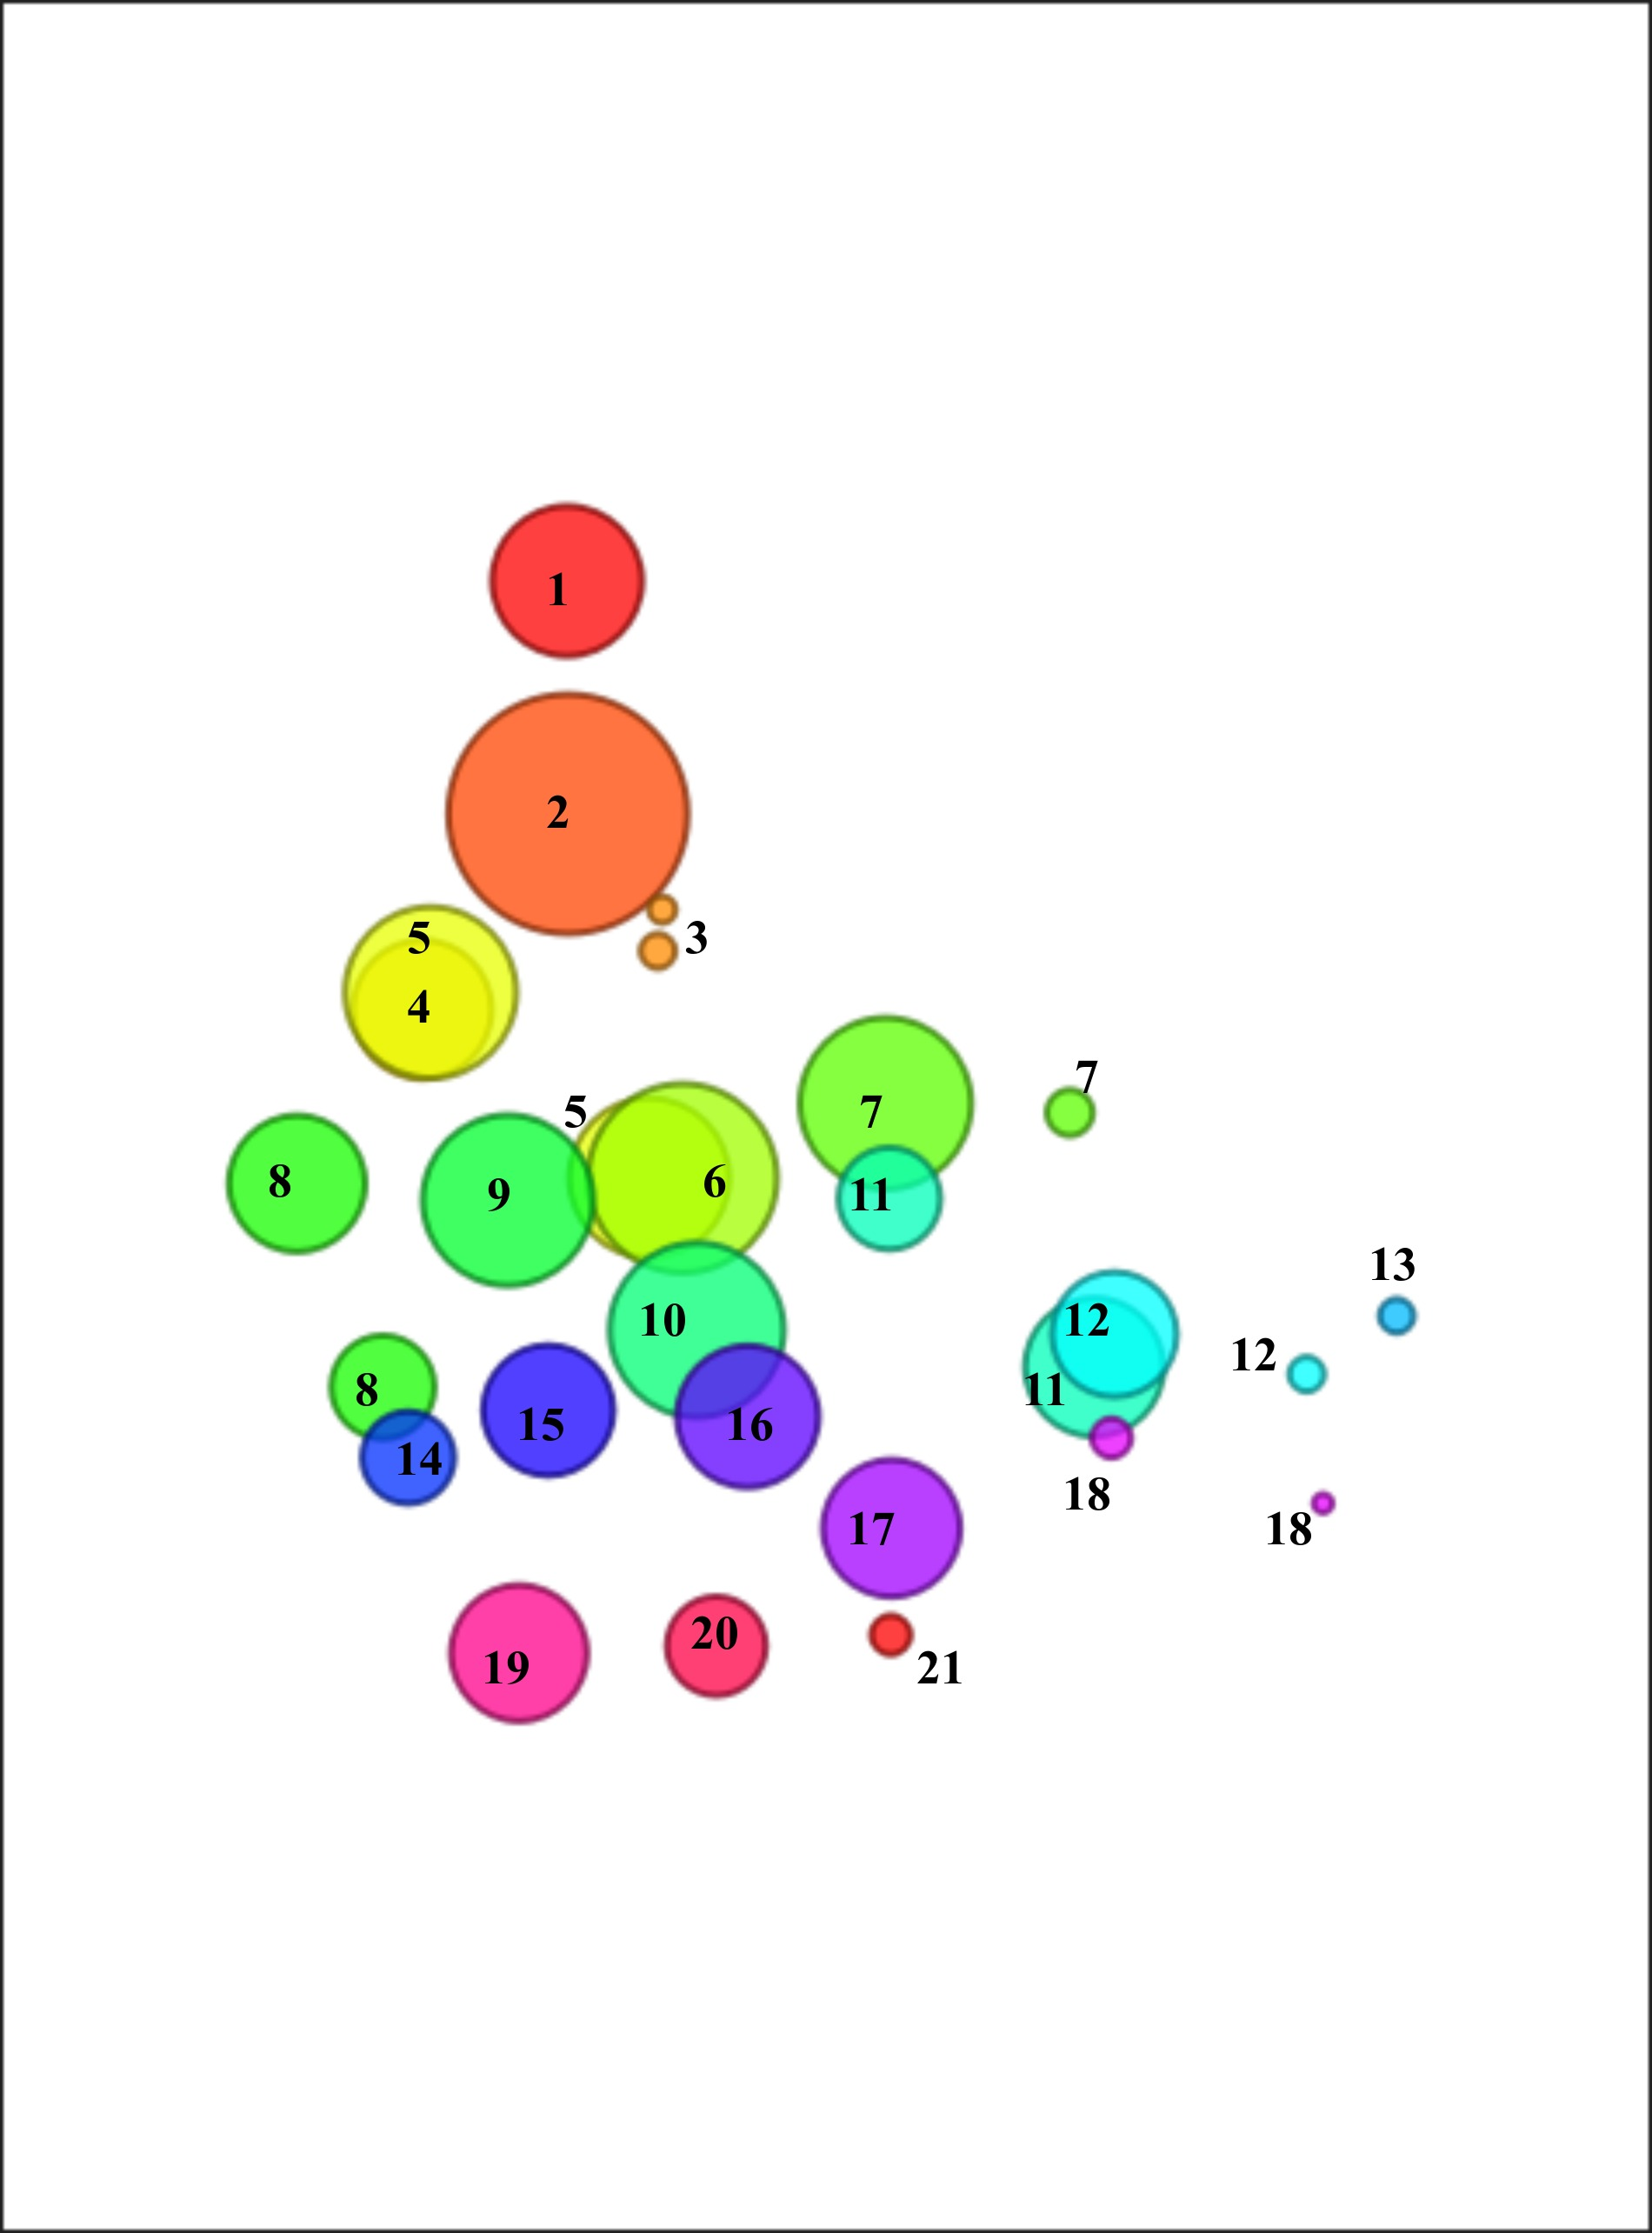
\includegraphics[width=0.7\columnwidth]{figs/engine-block-clusters-tf.jpg}
    \caption{Volume exploration space for the engine block dataset. Method parameters setup: transfer function $=\{$intensity, skewness, gradient magnitude and variance$\}$; $minPts = 4$;  $\varepsilon = 0.35$; and $\alpha = 0.85$.}
    \label{fig:engine-block-clusters-tf}
\end{figure}

\begin{figure}[htb!]
    \centering
    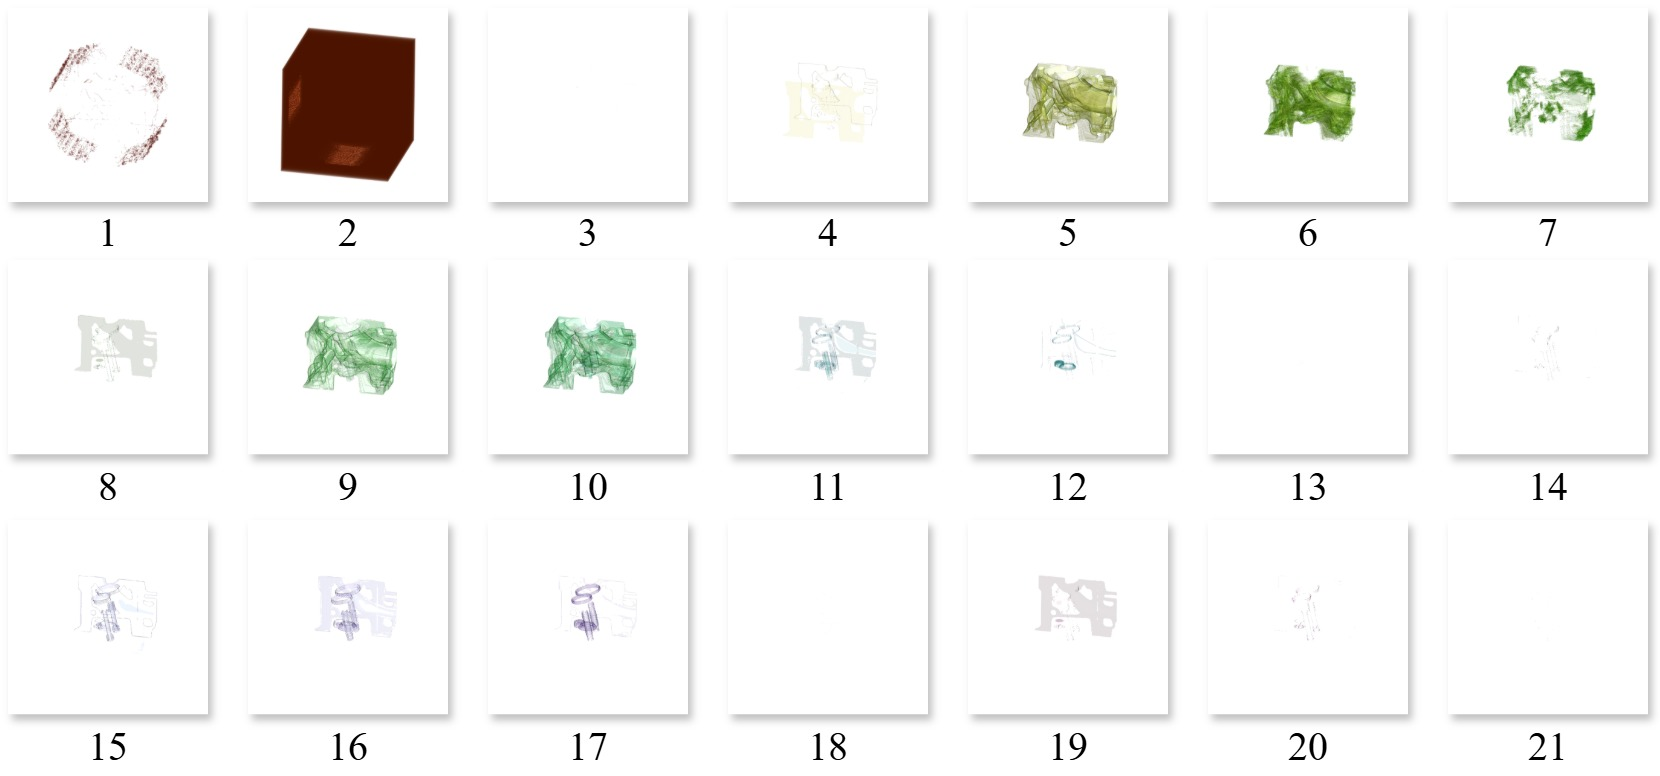
\includegraphics[width=\columnwidth]{figs/engine-block-clusters.jpg}
    \caption{Rendered volume classification details for the engine block dataset. Method parameters setup: transfer function  $=\{$intensity, skewness, gradient magnitude and variance$\}$; $minPts = 4$; $\varepsilon = 0.35$; and $\alpha = 0.85$.}
    \label{fig:engine-block-clusters}
\end{figure}

A volume exploration simulation is demonstrated in Fig.~\ref{fig:engine-block-groups}. It reveals different engine block components. The process happens from the initial setup presented in Fig.~\ref{fig:engine-block-clusters-tf}. 

\begin{figure}[htb!]
    \centering
    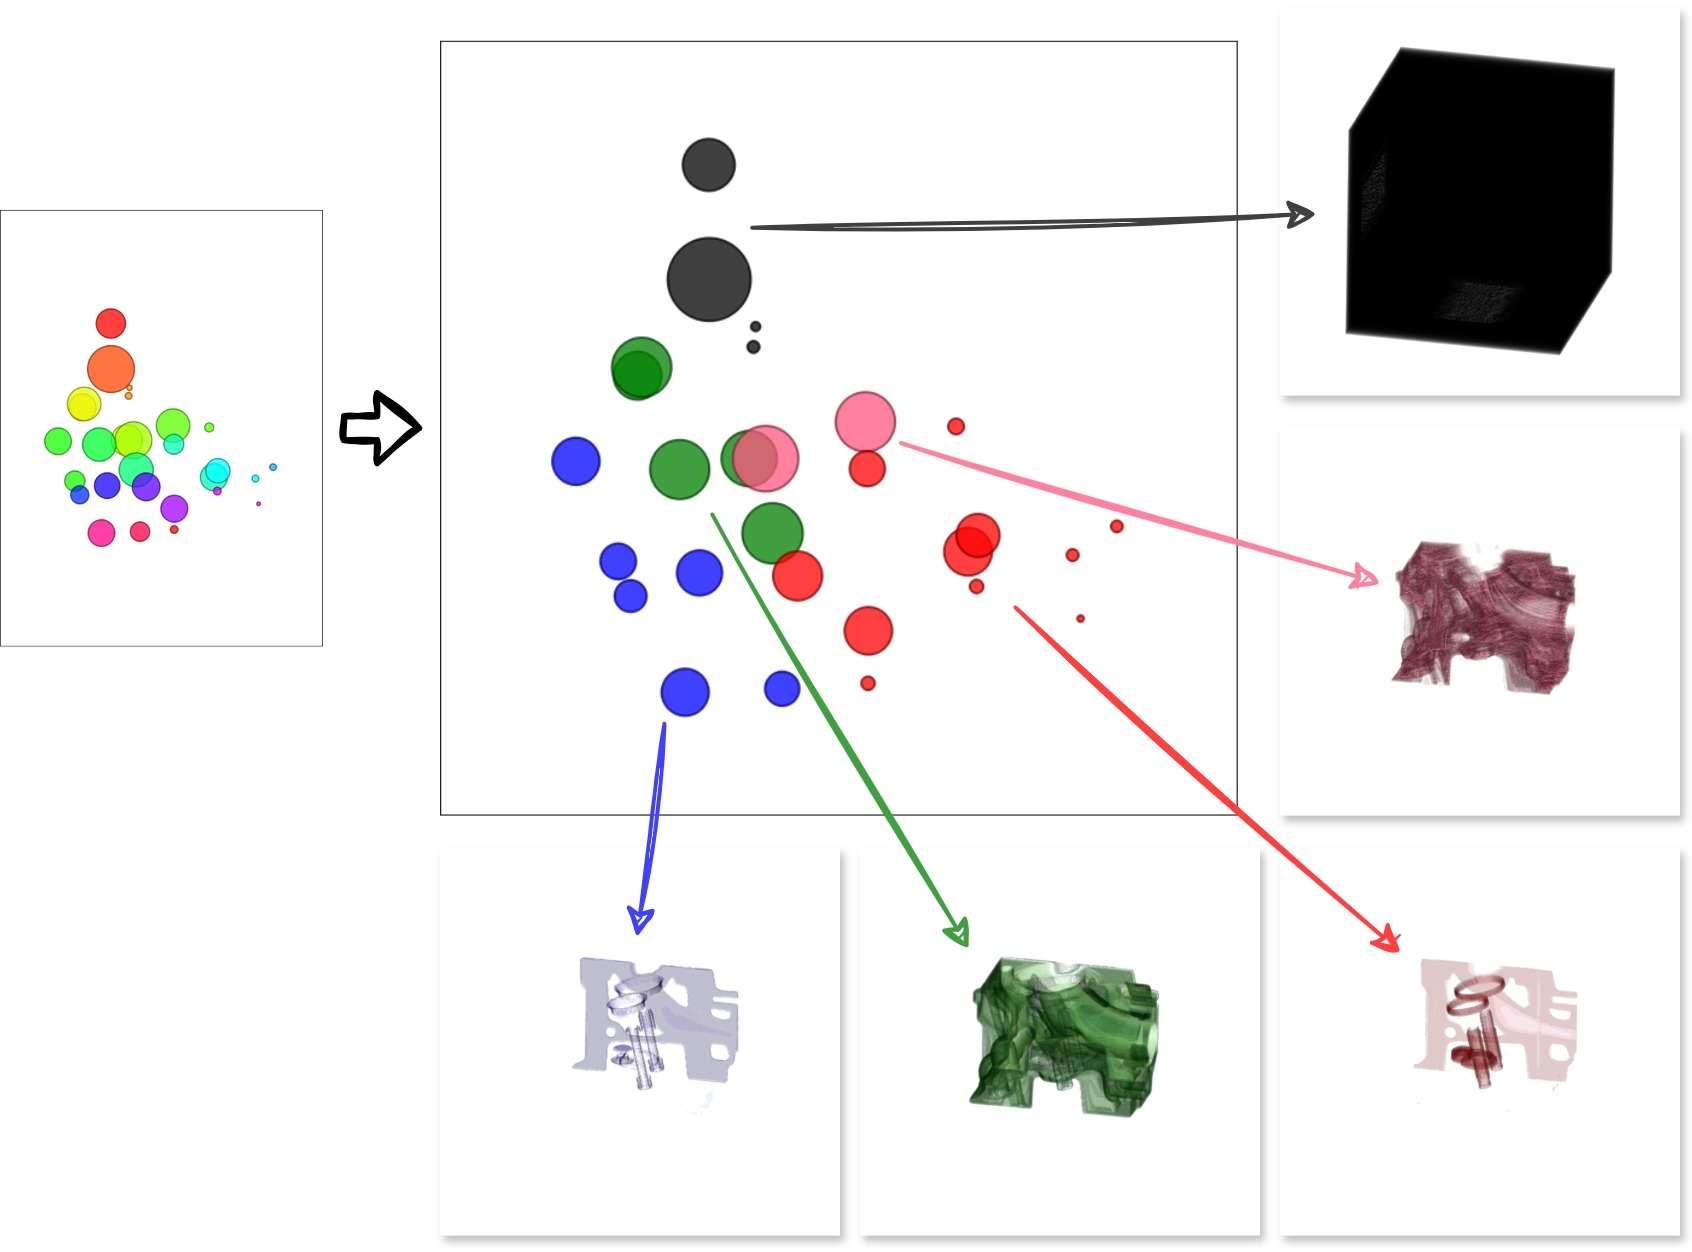
\includegraphics[width=\columnwidth]{figs/engine-block-groups.jpg}
    \caption{Visual analysis of user-refined transfer function design and volume classification for engine block datasets. The volume details are manually grouped from an empirical perspective. Method parameters setup: transfer function $=\{$intensity, skewness, gradient magnitude and variance$\}$; $minPts = 4$; $\varepsilon = 0.35$; and $\alpha = 0.85$.}
    \label{fig:engine-block-groups}
\end{figure}



\subsubsection{Knees dataset}
\label{subsubsect:knees-dataset}
A preliminary volume classification for knees datasets is presented in Fig.~\ref{fig:knees-tf-clusters} and the related rendered details in Fig.~\ref{fig:knees-clusters}. The method parameters are set as follows:  TF $=\{$intensity,  variance, absolute deviation, energy and contrast$\}$; $minPts = 4$; $\varepsilon = 0.35$; and $\alpha = 0.9$. 


\begin{figure}[htb!]
    \centering
    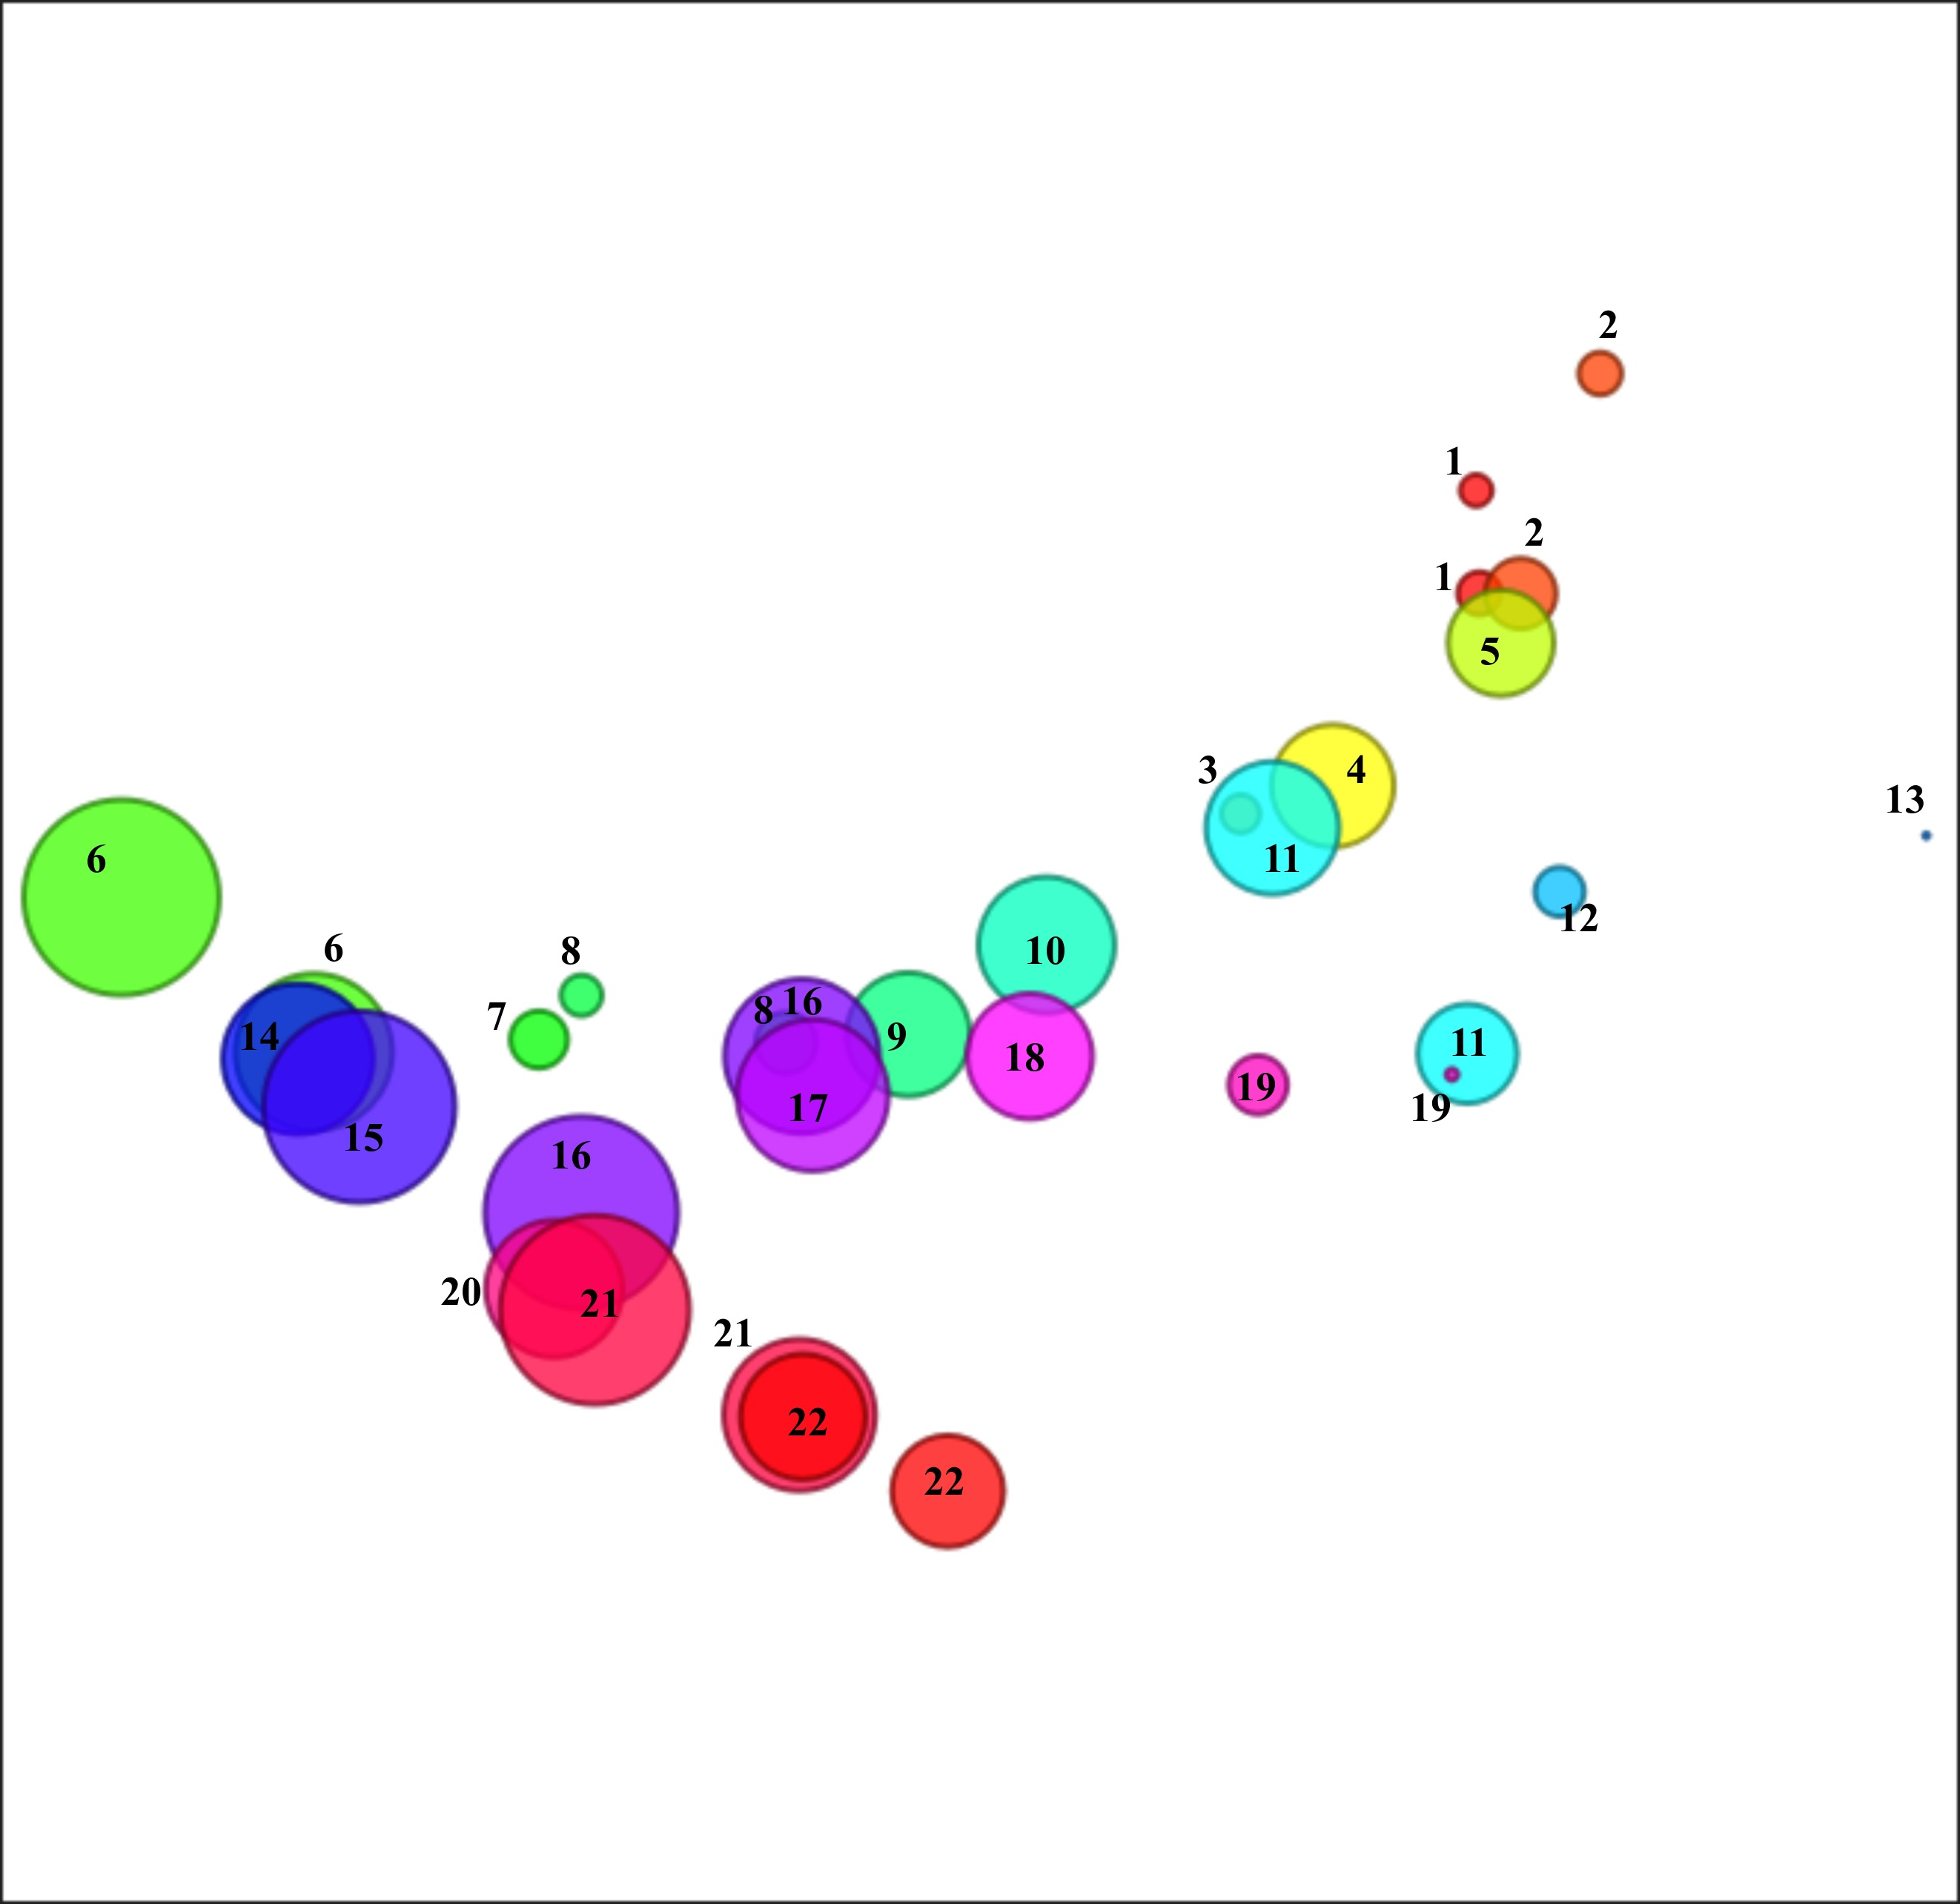
\includegraphics[width=0.7\columnwidth]{figs/knees-clusters-tf.jpg} 
     \caption{Volume exploration space for the knees dataset. Method parameters setup: transfer function $=\{$intensity,  variance, absolute deviation, energy and contrast$\}$; $minPts = 4$; $\varepsilon = 0.35$; and $\alpha = 0.9$.}
    \label{fig:knees-tf-clusters}
\end{figure}

\begin{figure}[htb!]
    \centering
    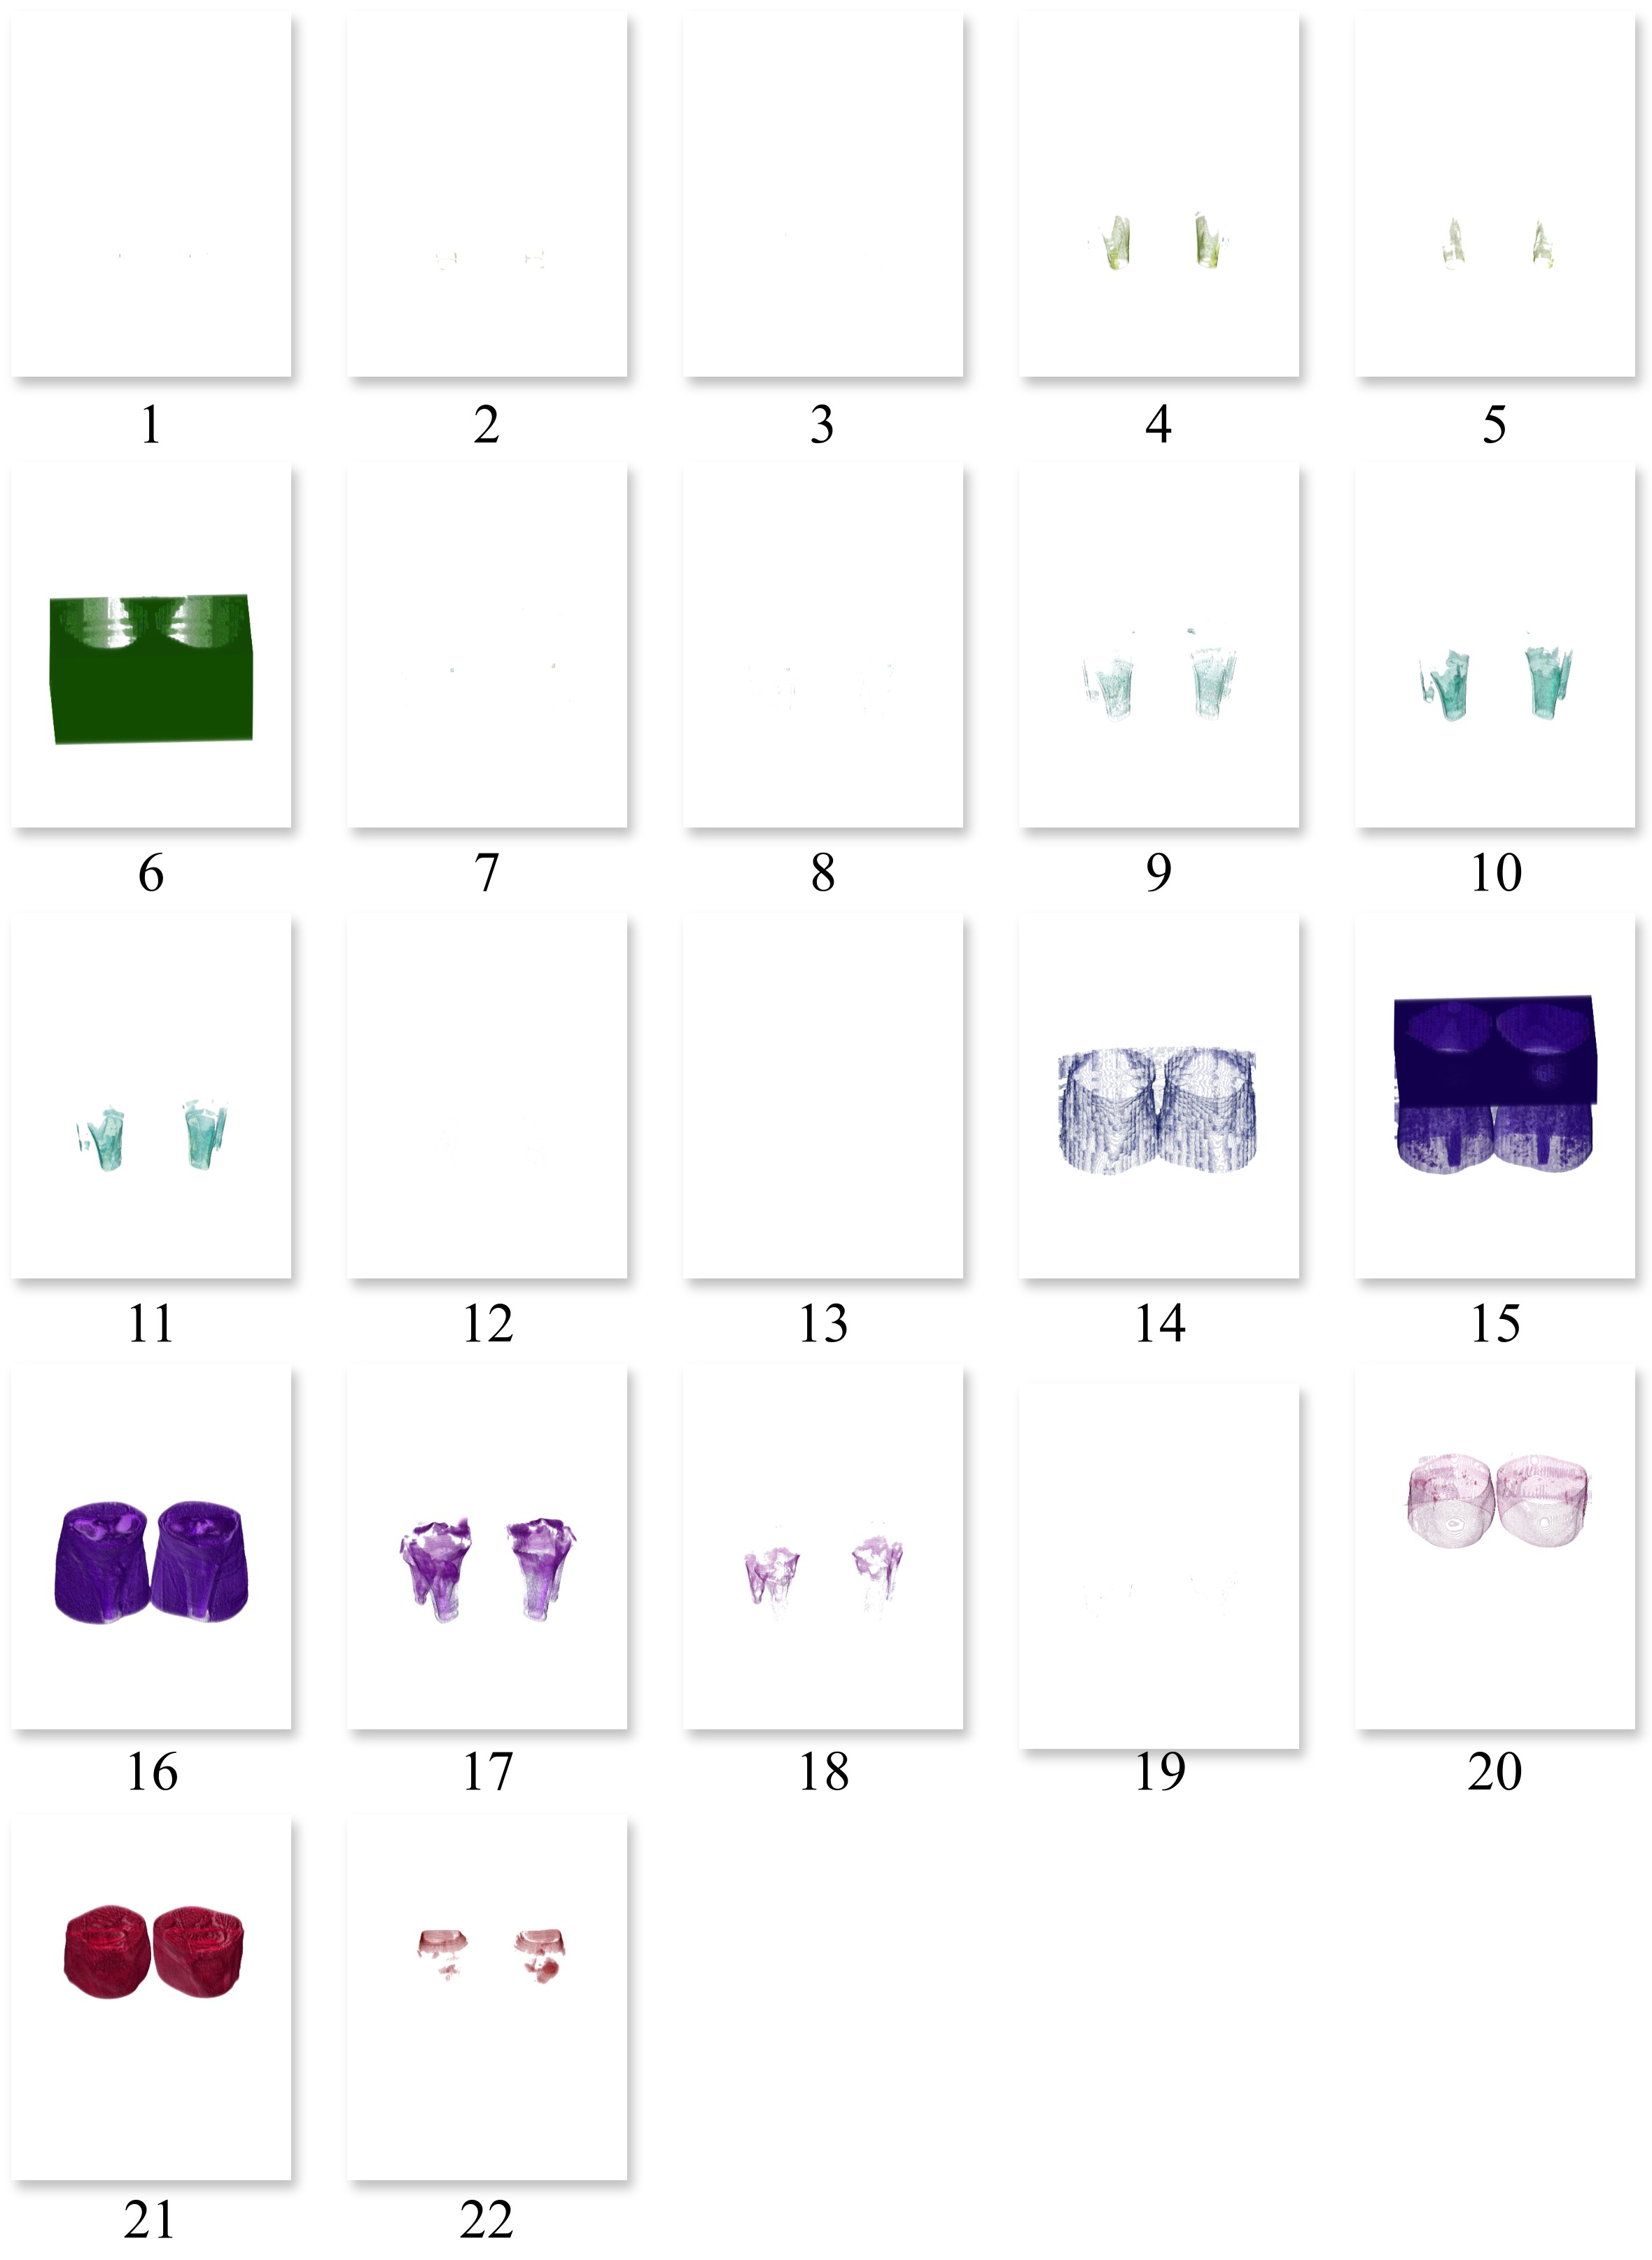
\includegraphics[width=\columnwidth]{figs/knees-clusters.jpg} 
     \caption{Rendered volume classification details for the knees dataset. Method parameters setup: transfer function $=\{$intensity,  variance, absolute deviation, energy and contrast$\}$; $minPts = 4$; $\varepsilon = 0.35$; and $\alpha = 0.9$.}
    \label{fig:knees-clusters}
\end{figure}


By exploring the volume details, it is possible to group and identify bones and muscular structures. Fig.~\ref{fig:knees-groups} illustrates these structures, which include parts of the femur, tibia, patella, fibula, thigh muscles, and knee muscles.

\begin{figure}[htb!]
    \centering
    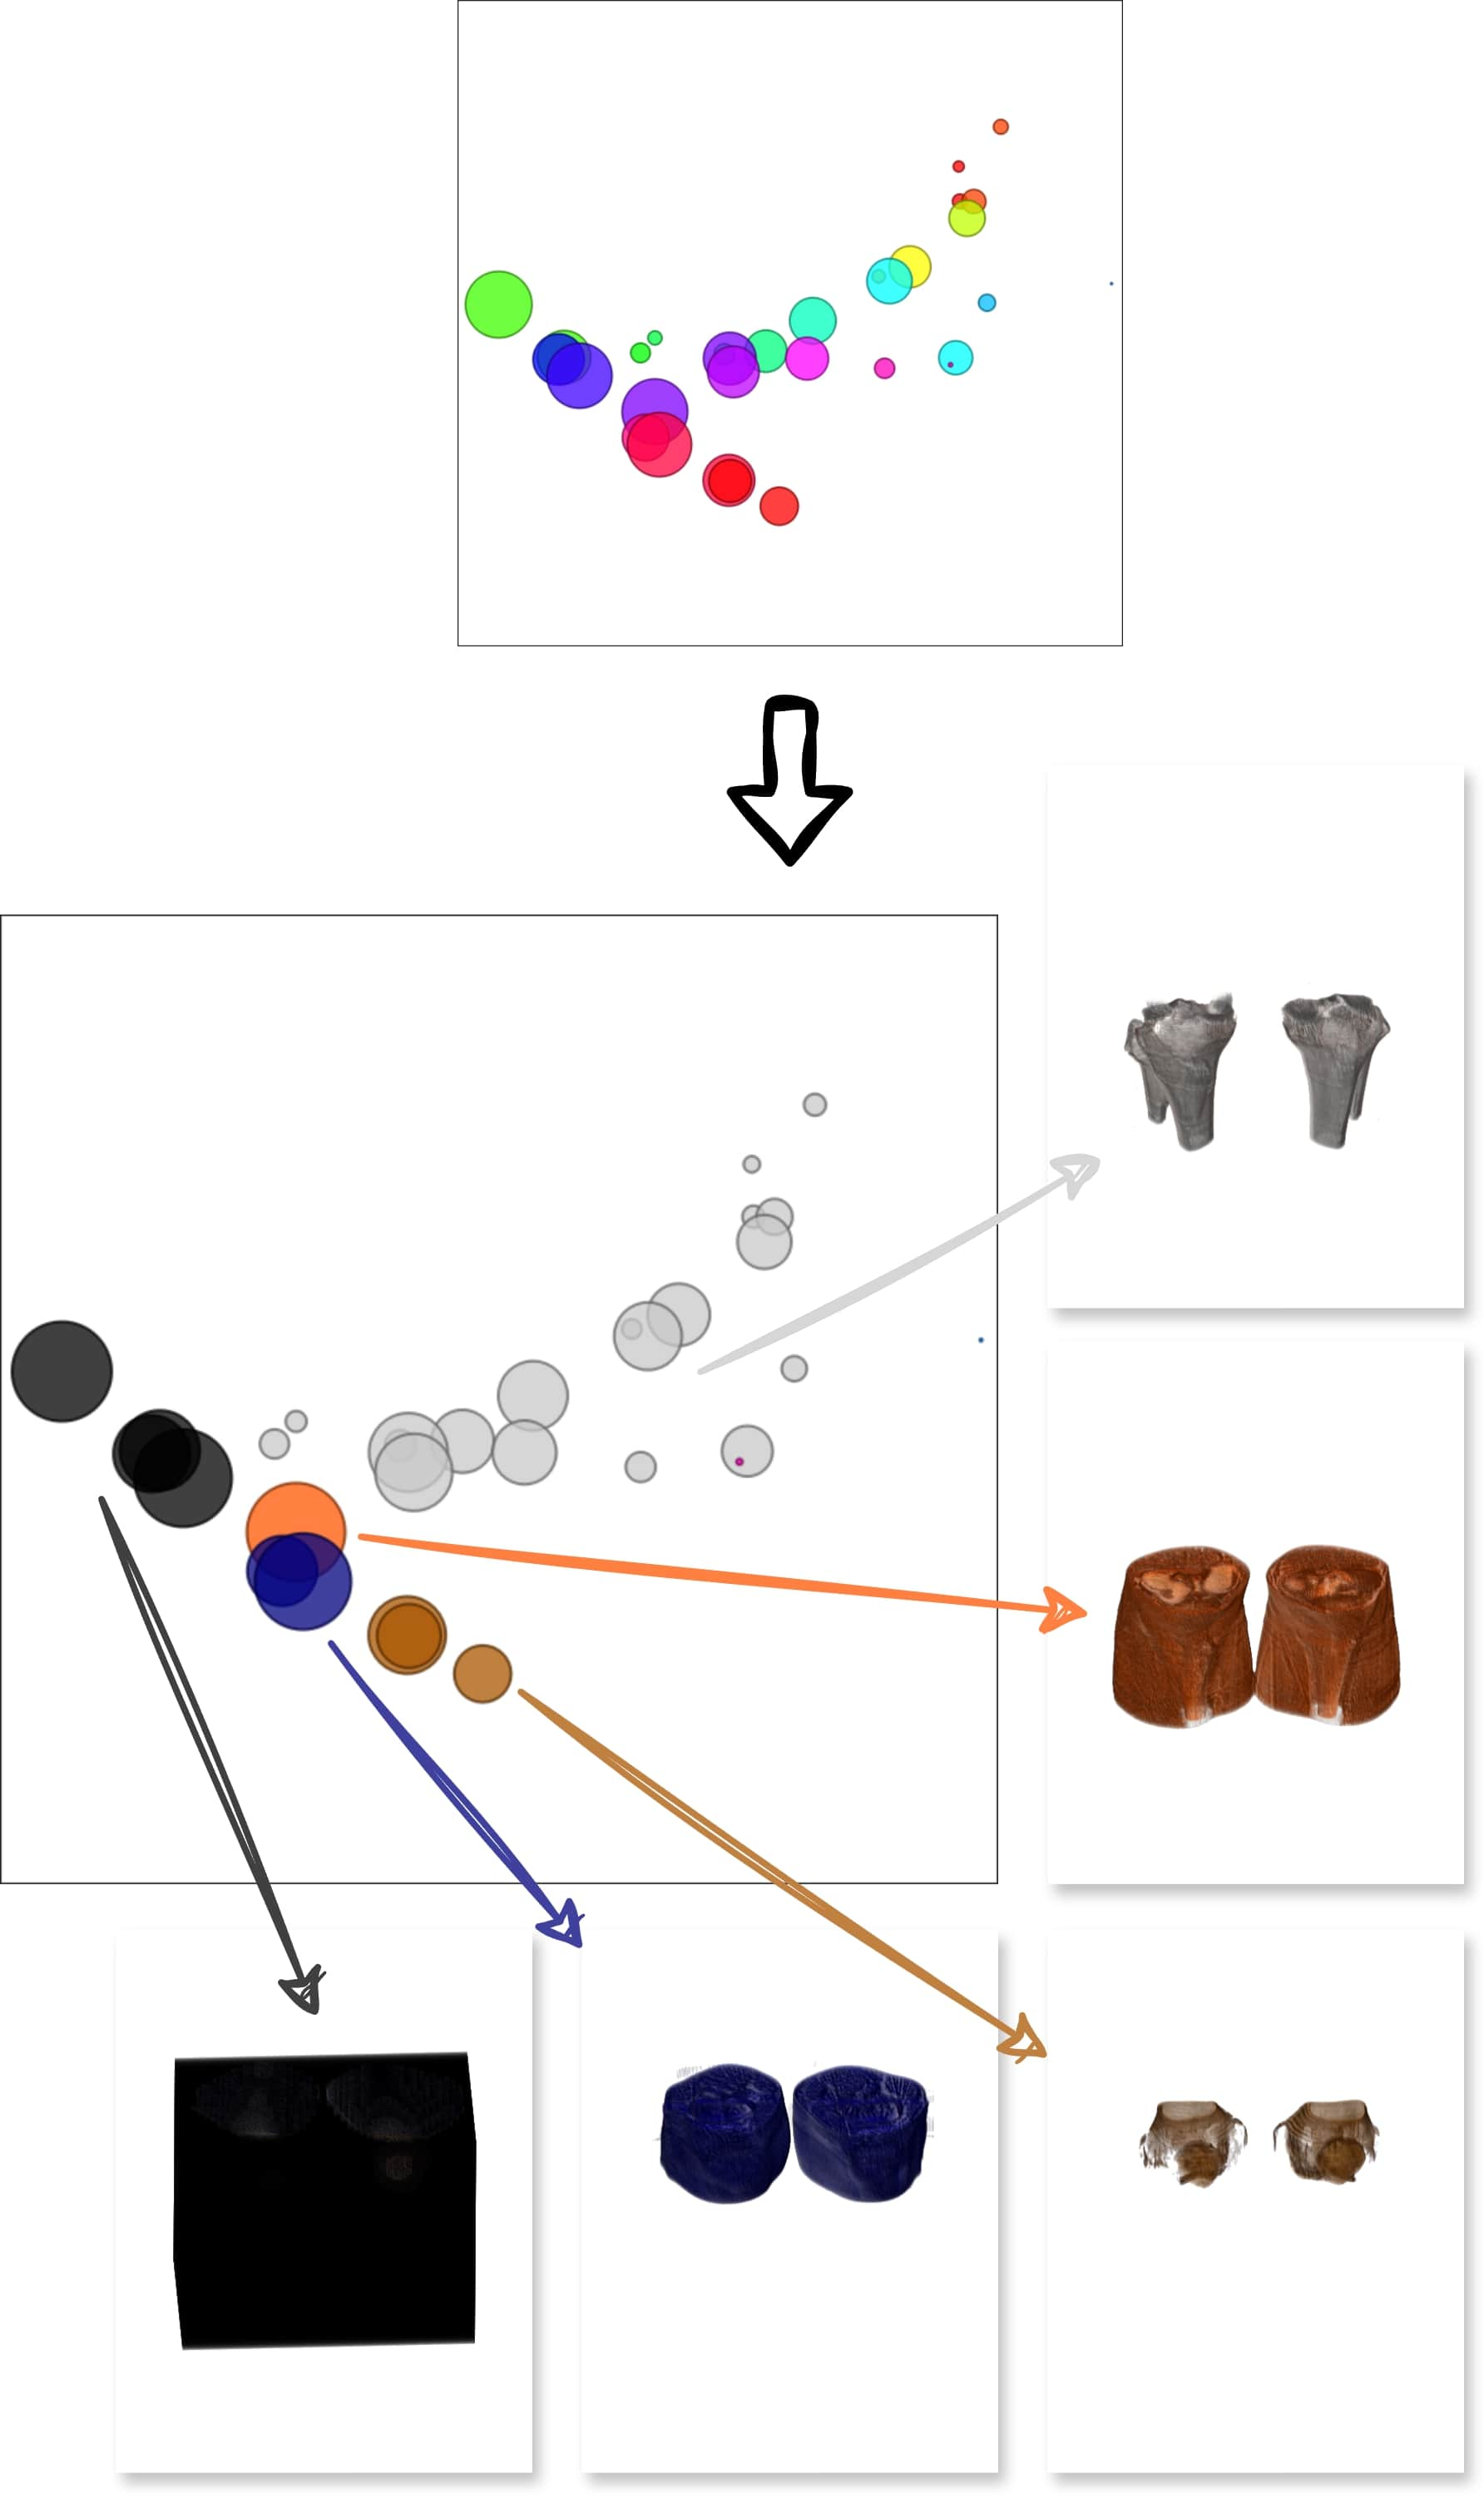
\includegraphics[width=\columnwidth]{figs/knees-groups.jpg}
    \caption{Visual analysis of user-refined transfer function design and volume classification for knees dataset. The volume details are manually grouped from an empirical perspective. Method parameters setup: transfer function $=\{$intensity,  variance, absolute deviation, energy and contrast$\}$; $minPts = 4$; $\varepsilon = 0.35$; and $\alpha = 0.9$.}
    \label{fig:knees-groups}
\end{figure}




\subsubsection{Tooth dataset}
\label{subsubsect:tooth-dataset}
Fig.~\ref{fig:tooth-clusters} presents  visualizations of a tooth dataset classification. The method parameters are set as follows:  TF $= \{$intensity, variance, absolute deviation, energy, contrast and entropy$\}$; $minPts = 4$; $\varepsilon = 0.23$; and $\alpha = 0.9$.

\begin{figure}[htb!]
    \centering
    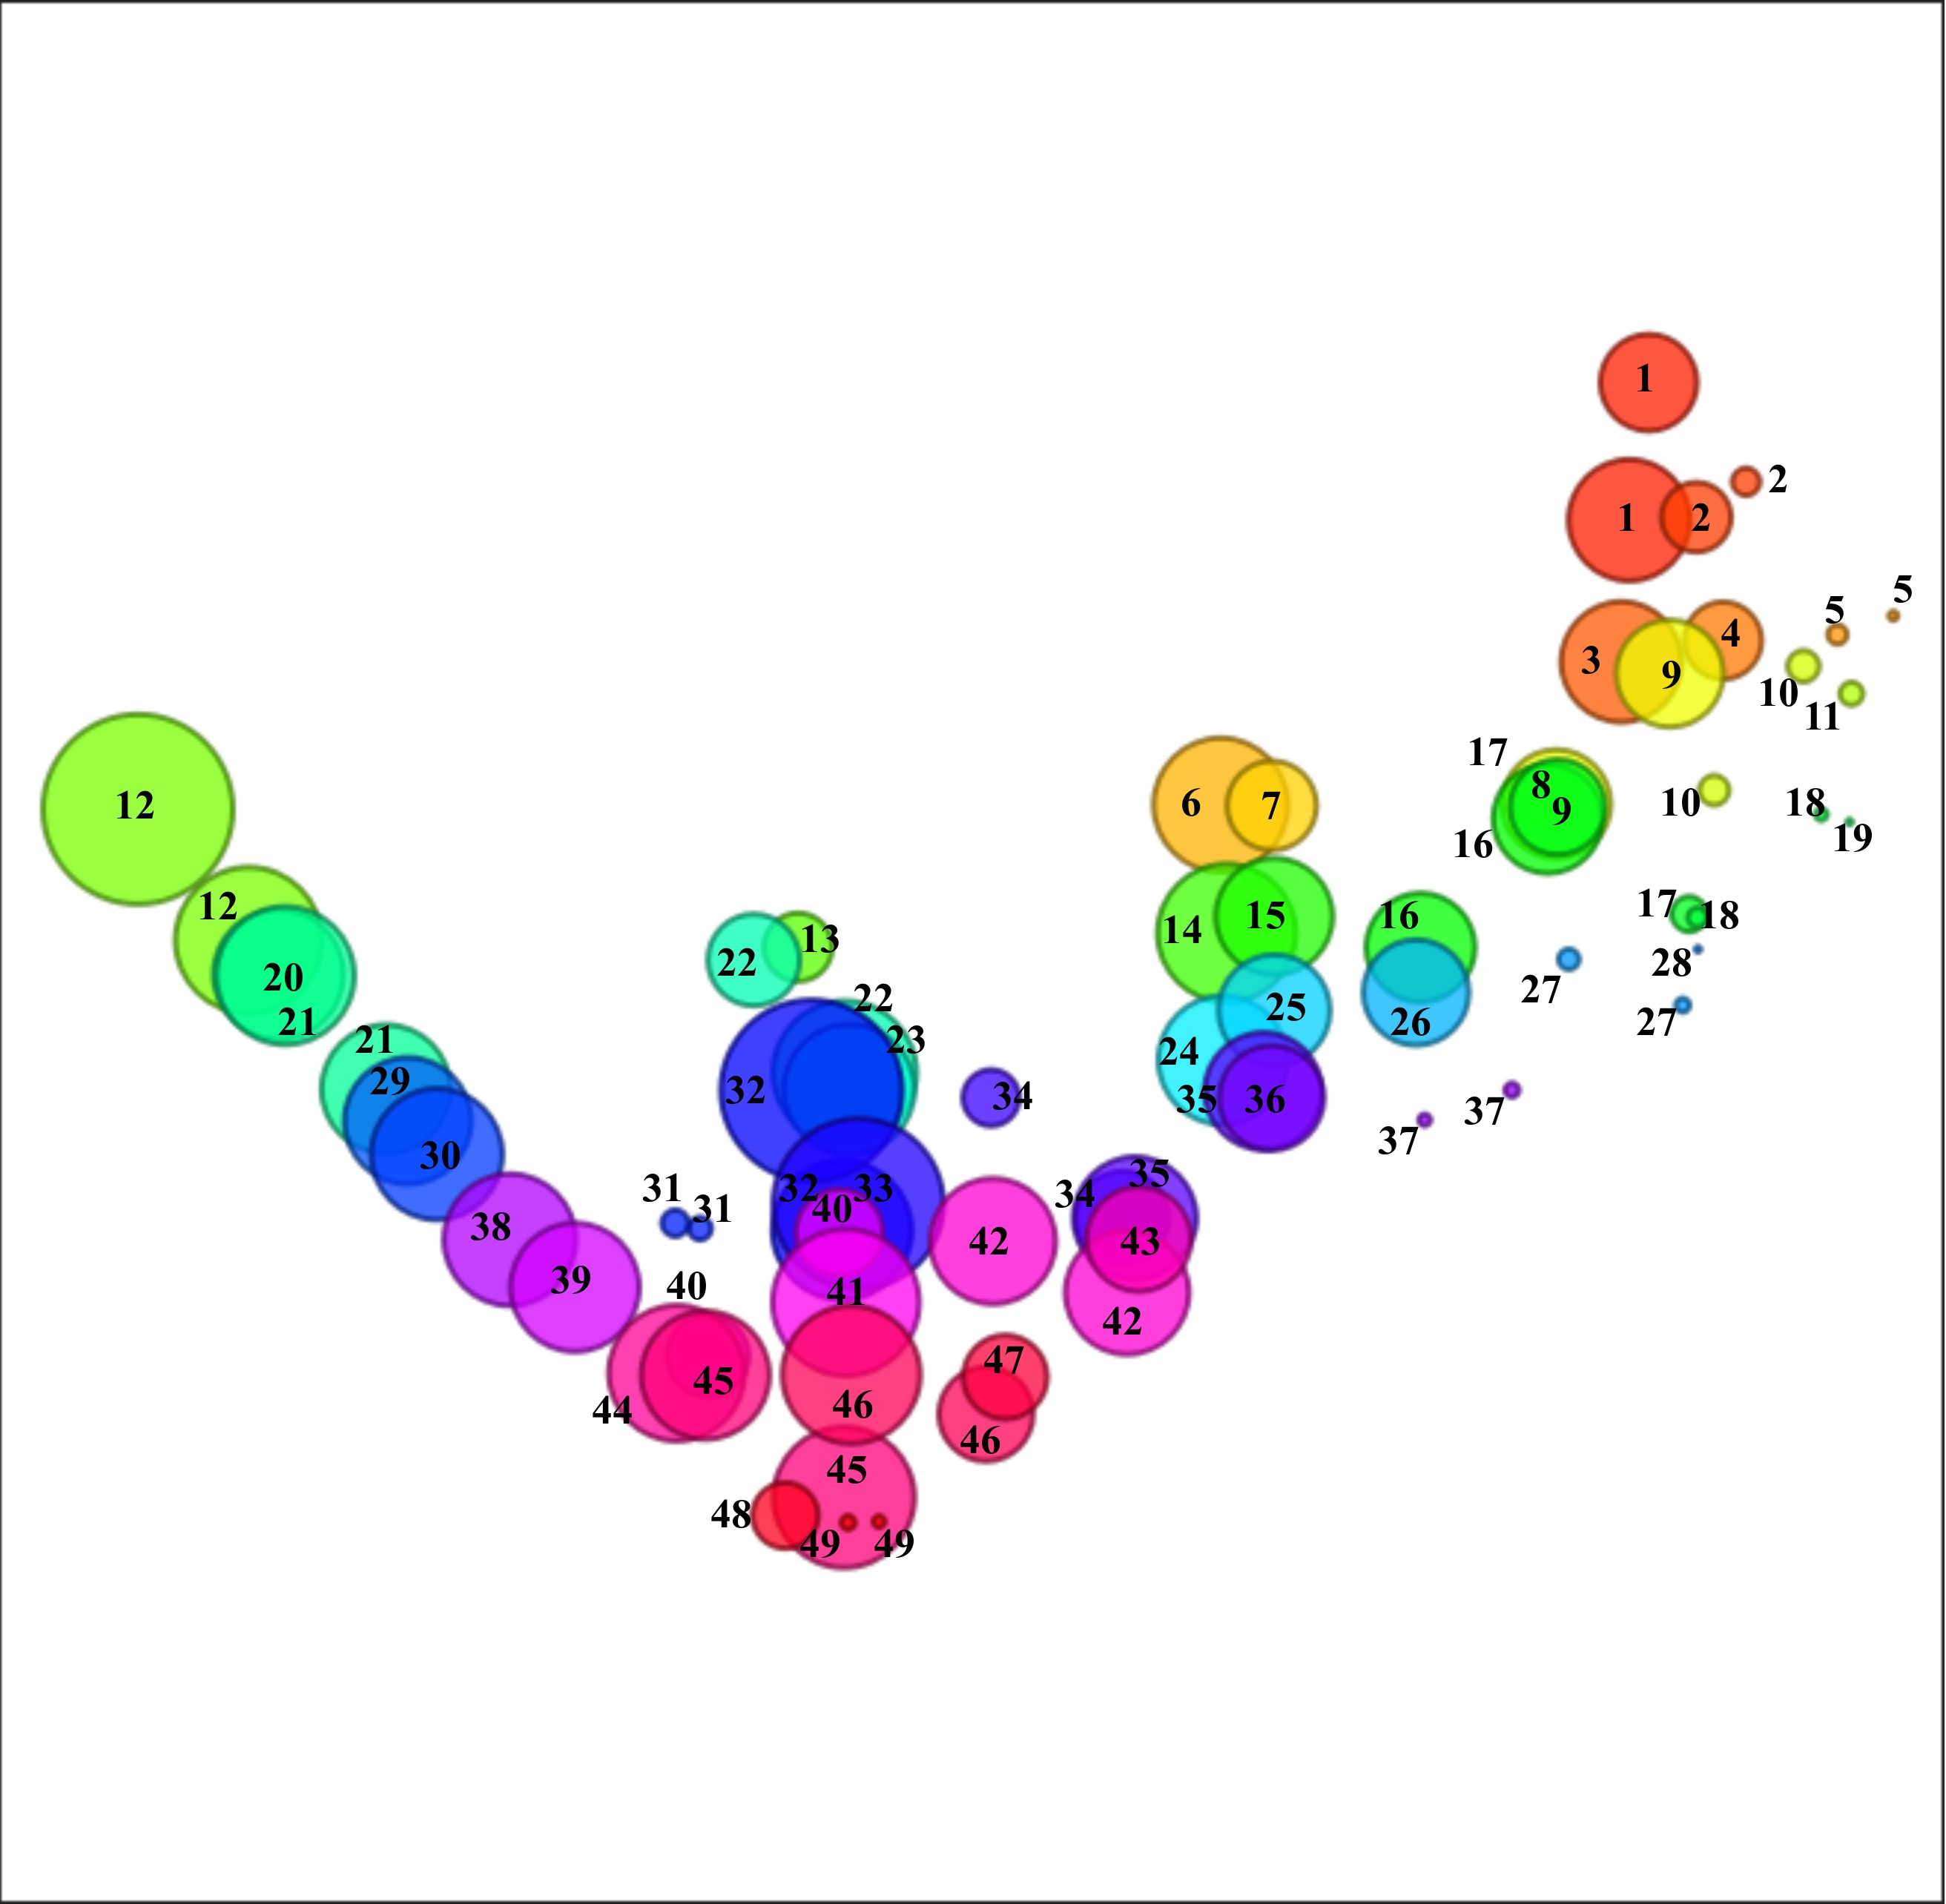
\includegraphics[width=0.7\columnwidth]{figs/tooth-clusters-tf.jpg} 
    \caption{Volume exploration space for the tooth dataset. Method parameters setup: transfer function $ =\{$intensity, variance, absolute deviation, energy, contrast and entropy$\}$; $minPts = 4$; $\varepsilon = 0.23$; and $\alpha = 0.9$.}
    \label{fig:tooth-clusters}
\end{figure}

\begin{figure}[htb!]
    \centering
    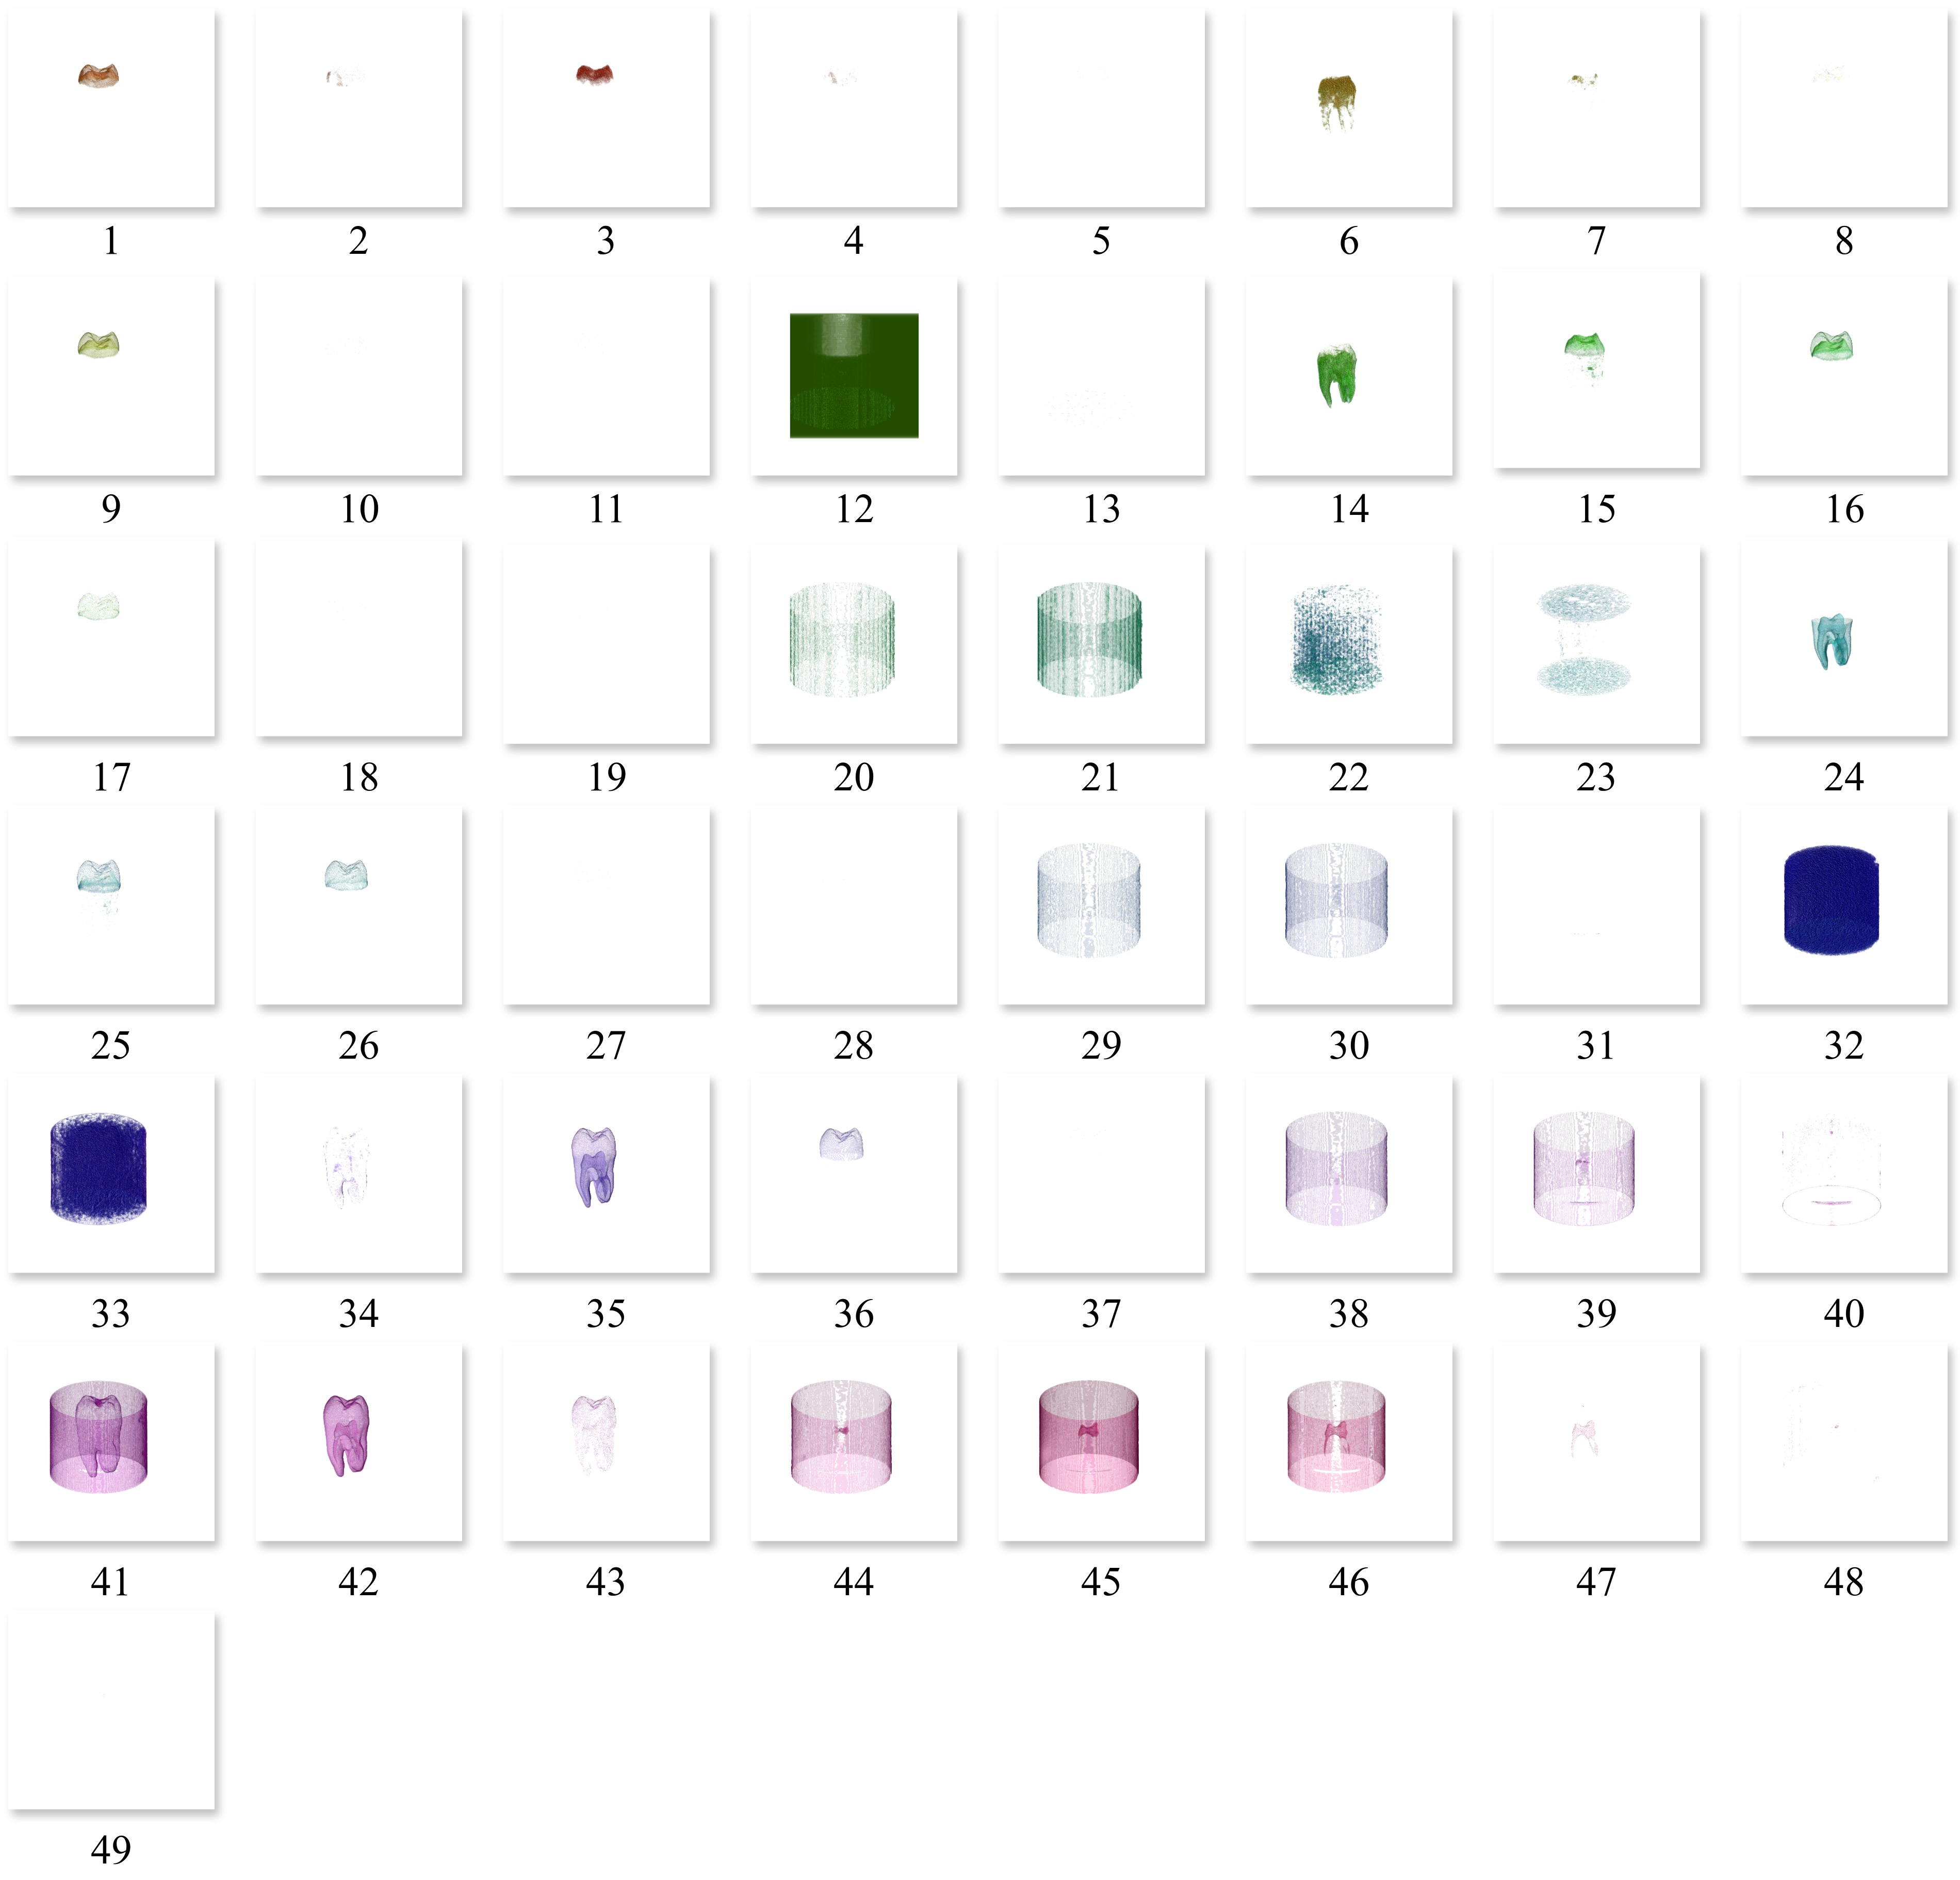
\includegraphics[width=\columnwidth]{figs/tooth-clusters.jpg} 
    \caption{Rendered volume classification details for the tooth dataset. The method parameters are set as follows: transfer function $ =\{$intensity, variance, absolute deviation, energy, contrast and entropy$\}$; $minPts = 4$; $\varepsilon = 0.23$; and $\alpha = 0.9$.}
    \label{fig:tooth-clusters}
\end{figure}


Manually generated groups of related tooth details are presented in Fig.~\ref{fig:tooth-groups}.  It shows several discernible structures, including the enamel, pulp, dentin, crown, the entire tooth, and the fluid in which it is immersed.

\begin{figure}[htb!]
    \centering
    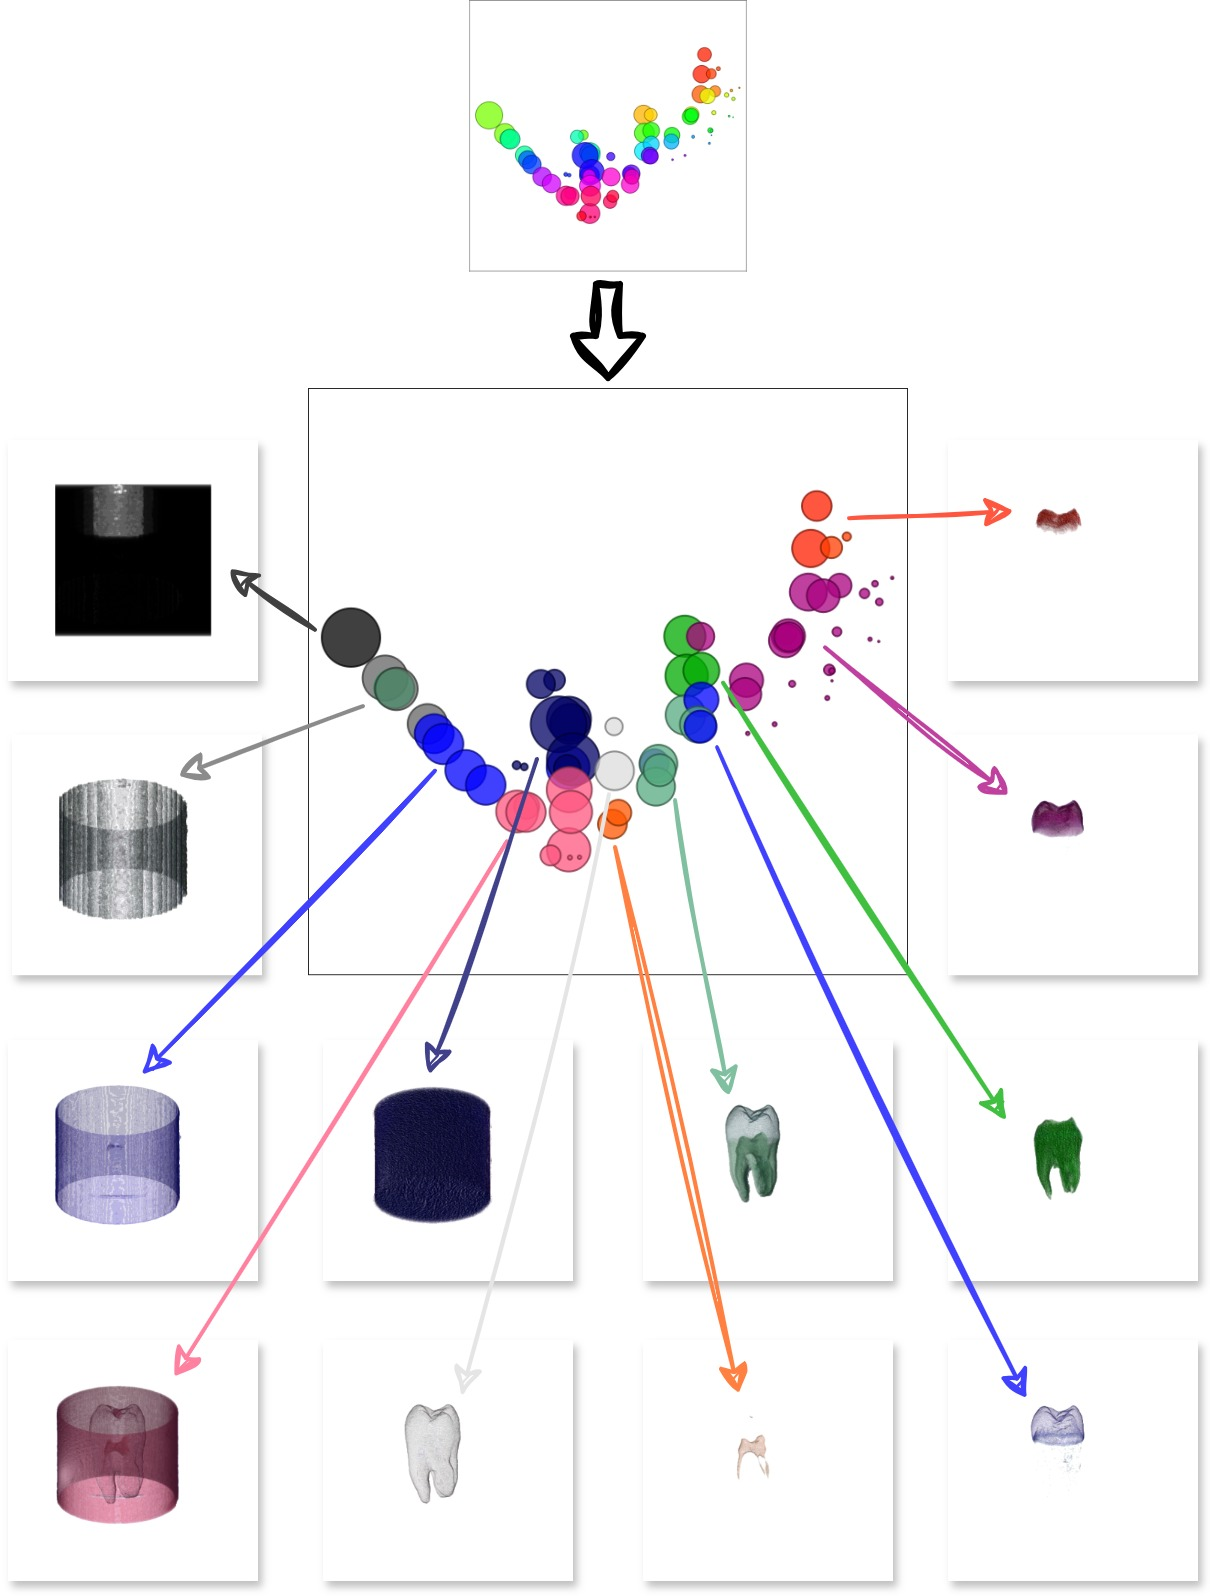
\includegraphics[width=\columnwidth]{figs/tooth-groups.jpg}
    \caption{Visual analysis of user-refined transfer function design and volume classification for tooth dataset. The volume details are manually grouped from an empirical perspective. The method parameters are set as follows: transfer function domain $ =\{$intensity, variance, absolute deviation, energy, contrast and entropy$\}$; $minPts = 4$; $\varepsilon = 0.23$; and $\alpha = 0.9$.}
    \label{fig:tooth-groups}
\end{figure}